\documentclass[german=true,thesistype=bachelor,nolistoffigures,nodate]{tubsthesis}

\usepackage{lipsum}

\thesisname{Johanna Doe}
\thesismatrikel{1234567}
\thesisemail{j.doe@tu-braunschweig.de}
\thesismajor{Informatik}
\thesisduration{3}
\thesissupervisors{Super Visor, M. Sc.}{Dr. Dipper Visor}{}
\thesisprofessor[Prof.\,Dr.-Ing.\,Jane Smith]{Prof.\,Dr.-Ing.\,Lars Eisbär}
\thesistitle{Titel der Thesis}{Title of the thesis}
\thesisbegindate{2020-01-01}
%\thesisenddate{2020-01-02}
\thesispresentationpoints{5.7}

\addbibresource{bibliography.bib}

\thesisinstitute{Institut für Perfektes Schreiben in IT}

\begin{document}
    \thesisabstract[%
        This is an english text.\\
        \lipsum[1-2]
    ]{%
        Hier steht ein Text auf Deutsch.\\
        \lipsum[3-4]
    }

    \begin{thesis}

        \chapter{Einleitung}

        \lipsum[1-3]
        \begin{table}[h]
            \centering
            \begin{tabular}{c|c|c|c|c}
            1 & 0 & 0 & 0 & 1 \\
            1 & 0 & 0 & 0 & 0 \\
            0 & 0 & 1 & 1 & 1 \\
            1 & 1 & 0 & 1 & 1
            \end{tabular}
            \caption[Wichtige Tabelle]{Hierbei handelt es sich um eine wichtige Tabelle}
            \label{tab:important}
        \end{table}

        \begin{figure}
        \centering
        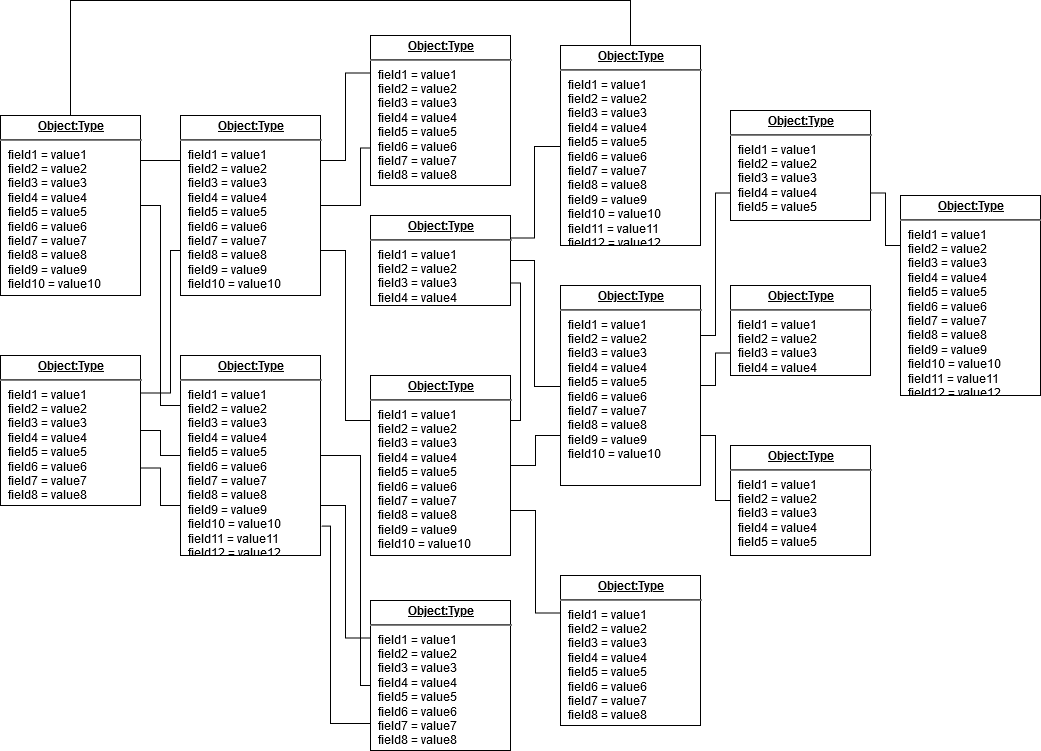
\includegraphics[width=\textwidth]{images/example_diagram.png}
        \caption{Ein Diagramm, nicht relevant für irgendetwas~\cite{lisa}}
        \label{fig:inga}
        \end{figure}

        \lipsum[4-7]

    \end{thesis}

    \chapter{Speichermedium}
    Hier gehört eine Tabelle des Inhalts deines beigefügten Speichermediums (SD-Karte/USB-Stick) hin.
    Ggf. müssen Kommentare/Erklärungen dazu geschrieben werden.
\end{document}